% 
% Copyright LANL 
% 
% This is documentation for the cinema file specification  
% 
 
\documentclass{article} 
 
\usepackage[export]{adjustbox} 
\usepackage{authblk} 
\usepackage[small,bf]{caption} 
\usepackage{cite} 
\usepackage{enumitem} 
\setlist[description]{leftmargin=\parindent,labelindent=\parindent} 
\usepackage{fancyhdr} 
\usepackage{graphicx} 
\usepackage[margin=1in]{geometry} 
\usepackage{pdfpages} 
\usepackage{tcolorbox} 
\usepackage{times} 
\usepackage{verbatim} 
\usepackage{wallpaper}
\usepackage{xspace}
\usepackage{xcolor}
\usepackage{textcomp}
\usepackage{hyperref}

\newcommand{\camstatic}     {\texttt{\small static}\xspace}
\newcommand{\camphi}        {\texttt{\small phi-theta}\xspace}
\newcommand{\cphi}          {\texttt{\small phi}\xspace}
\newcommand{\ctheta}        {\texttt{\small theta}\xspace}
\newcommand{\camazimuth}    {\texttt{\small azimuth-elevation-roll}\xspace}
\newcommand{\camyaw}        {\texttt{\small yaw-pitch-roll}\xspace}
\newcommand{\metadata}      {\texttt{\small metadata}\xspace}
\newcommand{\parameter}     {\texttt{\small parameter}\xspace}
\newcommand{\valuemode}     {\texttt{\small value\_mode}\xspace}
\newcommand{\namepattern}   {\texttt{\small name\_pattern}\xspace}
\newcommand{\pose}          {\texttt{\small pose}\xspace}
\newcommand{\parameterlist} {\texttt{\small parameter\_list}\xspace}
\newcommand{\cameramodel}   {\texttt{\small camera\_model}\xspace}

\newcommand{\LAUR} {LA-UR-17-25072\xspace}
\newcommand{\insitu} {\textit{in situ}\xspace}
\newcommand{\CinemaSpecVersion} {v1.0\xspace}
\newcommand{\Simple} {\textit{Simple}\xspace}
\newcommand{\astaire} {Astaire\xspace}
\newcommand{\bacall} {Bacall\xspace}
\newcommand{\chaplin} {Chaplin\xspace}
\newcommand{\dietrich} {Dietrich\xspace}
\newcommand{\cdevemail}{\texttt{\small cinema-dev@lanl.gov}\xspace}
\newcommand{\cinemaemail}{\texttt{\small cinema@lanl.gov}\xspace}
\newcommand{\cinemawebsite}{\texttt{\small http://www.cinemascience.org}\xspace}
\newcommand{\datacsv}{\texttt{\small data.csv}\xspace}

% \newcommand{\todo}[1]{
% }

\newcommand{\todo}[1]{
    \addcontentsline{tdo}{todo}{\protect{#1}}
    \marginpar{\colorbox{white!90!black}{\textcolor{black}{
    \parbox{2.1cm}{\scriptsize\bf\raggedright #1}
    }}}
}


\pagestyle{fancy}
\fancyhf{}
\renewcommand{\headrulewidth}{0pt}
\cfoot{\thepage}

\newcommand{\version}[0]{1.2\xspace}

%---------------------------------------------------------------------
%	TITLE SECTION
%---------------------------------------------------------------------


\begin{document}

\renewcommand\Authands{ and } 
 
% these lines implement subsubsubsection 
\setcounter{secnumdepth}{5} 
\setcounter{tocdepth}{5} 
\newcommand{\subsubsubsection}[1]{\paragraph{#1}} 


% create the cover page
%---------------------------------------------------------------------
% Title page 
%---------------------------------------------------------------------
\ThisCenterWallPaper{1.0}{img/script_cover.png}
\thispagestyle{empty}

\begin{ttfamily}
\begin{center}
 \ \ \\
\vspace{1.0 in}
\begin{figure}[h!]
\centering

\includegraphics[height=0.5in]{img/cinema_logo_name}
\end{figure}
\vspace{1.0 in}
Cinema Database Specification \\
\dietrich Release v1.2\\
\bigskip
\begin{figure}[h!]
\centering
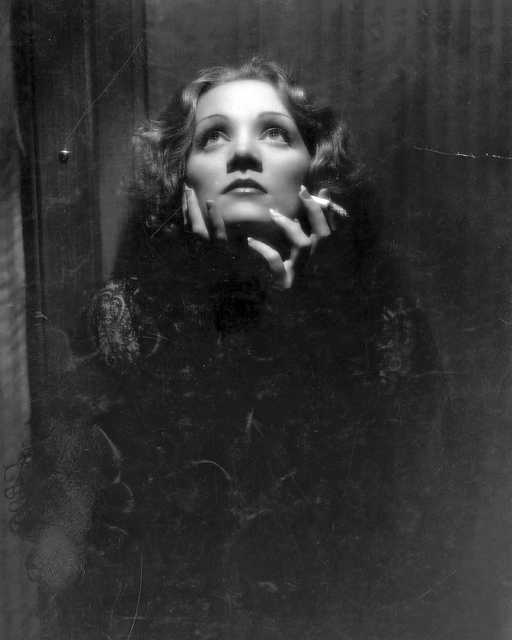
\includegraphics[height=1.0in]{img/dietrich_spec_logo}
\end{figure}
\bigskip
Document Version 1.1 \\
(September 2018)\\
\LAUR\\
\bigskip
\bigskip
\bigskip
\bigskip
by \\
\bigskip
David Rogers   \texttt{\small dhr@lanl.gov}\\
Jon Woodring   \texttt{\small woodring@lanl.gov}\\
James Ahrens   \texttt{\small ahrens@lanl.gov}\\
John Patchett  \texttt{\small patchett@lanl.gov}\\
Jonas Lukascyk \texttt{\small jl@jluk.de}\\
\end{center}
\vspace{1.0 in}
\begin{flushright}
Los Alamos National Laboratory\\
Bikini Atoll Rd., SM 30\\
Los Alamos, NM 87545\\
cinema@lanl.gov\\
\end{flushright}
\end{ttfamily}
\newpage

\tableofcontents
\newpage

\pagenumbering{arabic}


\section{Introduction}
\label{intro}
This document is a specification for Cinema databases. It is specification D
(\dietrich), version 1.1. This is a different approach than past specifications
\cite{cinemaSpecA}\cite{cinemaSpecC}, but is complimentary in spirit and
function to them. This version is a simple embodiment of the new approach,
which can be easily adapted to a wide range of use cases, and is designed for
quick adoption by scientists, programmers and others.

See the Cinema website (\cinemawebsite) for additional information, and contact
the Cinema community (\cinemaemail) or the authors of this document with
questions.


\section{Cinema Overview}
\label{overview}
\label{sec:cinema}

Extreme scale scientific simulations are leading a charge to exascale computation, and data analytics runs the risk of being a bottleneck to scientific discovery. Due to power and I/O constraints, we expect in situ visualization and analysis will be a critical component of these workflows. 

Options for extreme scale data analysis are often presented as a stark contrast: write large files to disk for interactive, exploratory analysis, or perform in situ analysis to save detailed data about phenomena that a scientist knows about in advance. Cinema represents a novel framework for a third option – a highly interactive, data artifact-based approach that promotes exploration of simulation results, and is easily accessed through database specifications. This approach supports interactive exploration of a wide range of results, while still significantly reducing data movement and storage.

More information about the overall design of Cinema is available in the paper \textit{An Image-based Approach to Extreme Scale In Situ Visualization and Analysis} \cite{cinemaSC14}.

A Cinema Database supports the following three use cases. Taken together, these support a novel method for interactively exploring artifacts from extremely large datasets.

\begin{enumerate}
\item Searching/querying of meta-data and data artifacts. Samples can be searched purely on metadata, content, position, time, or a combination of all of these.
\item Interactive visualization of sets of data artifacts.
\item Playing interactive visualizations, allowing the user on/off control of elements in the visualization.
\end{enumerate}

\subsection{What is a Cinema Database?}
A Cinema database is a set of precomputed data artifacts that can be queried and interactively viewed. The user can decide what types of components comprise the database, based on the type of interaction that is desired with the final database.
A general design philosophy of Cinema is that applications reading and viewing a Cinema database can ignore data and determine which operations to perform. This promotes a wide range of possible interactions with the data - not just the ones imagined by the creator of the database.

Previous Cinema database specifications have concentrated on the notion that a database is a set of results sampled by visualization parameters. In this specification, we abstract this to include typical use cases from experiments by scientists. 

A scientist often has a spreadsheet with data about parameters for an experiment. This results in a set of parameters that map to a particular result - a graph, a sensor image, or other image-based data. These are a natural abstraction from previous Cinema databases. Figure \ref{fig:parametersets} shows this mapping of parameter sets to results. A collection of these mappings can be easily expressed in a Cinema database, using this specification. This is detailed in later sections.

\begin{figure}[h!]
\centering
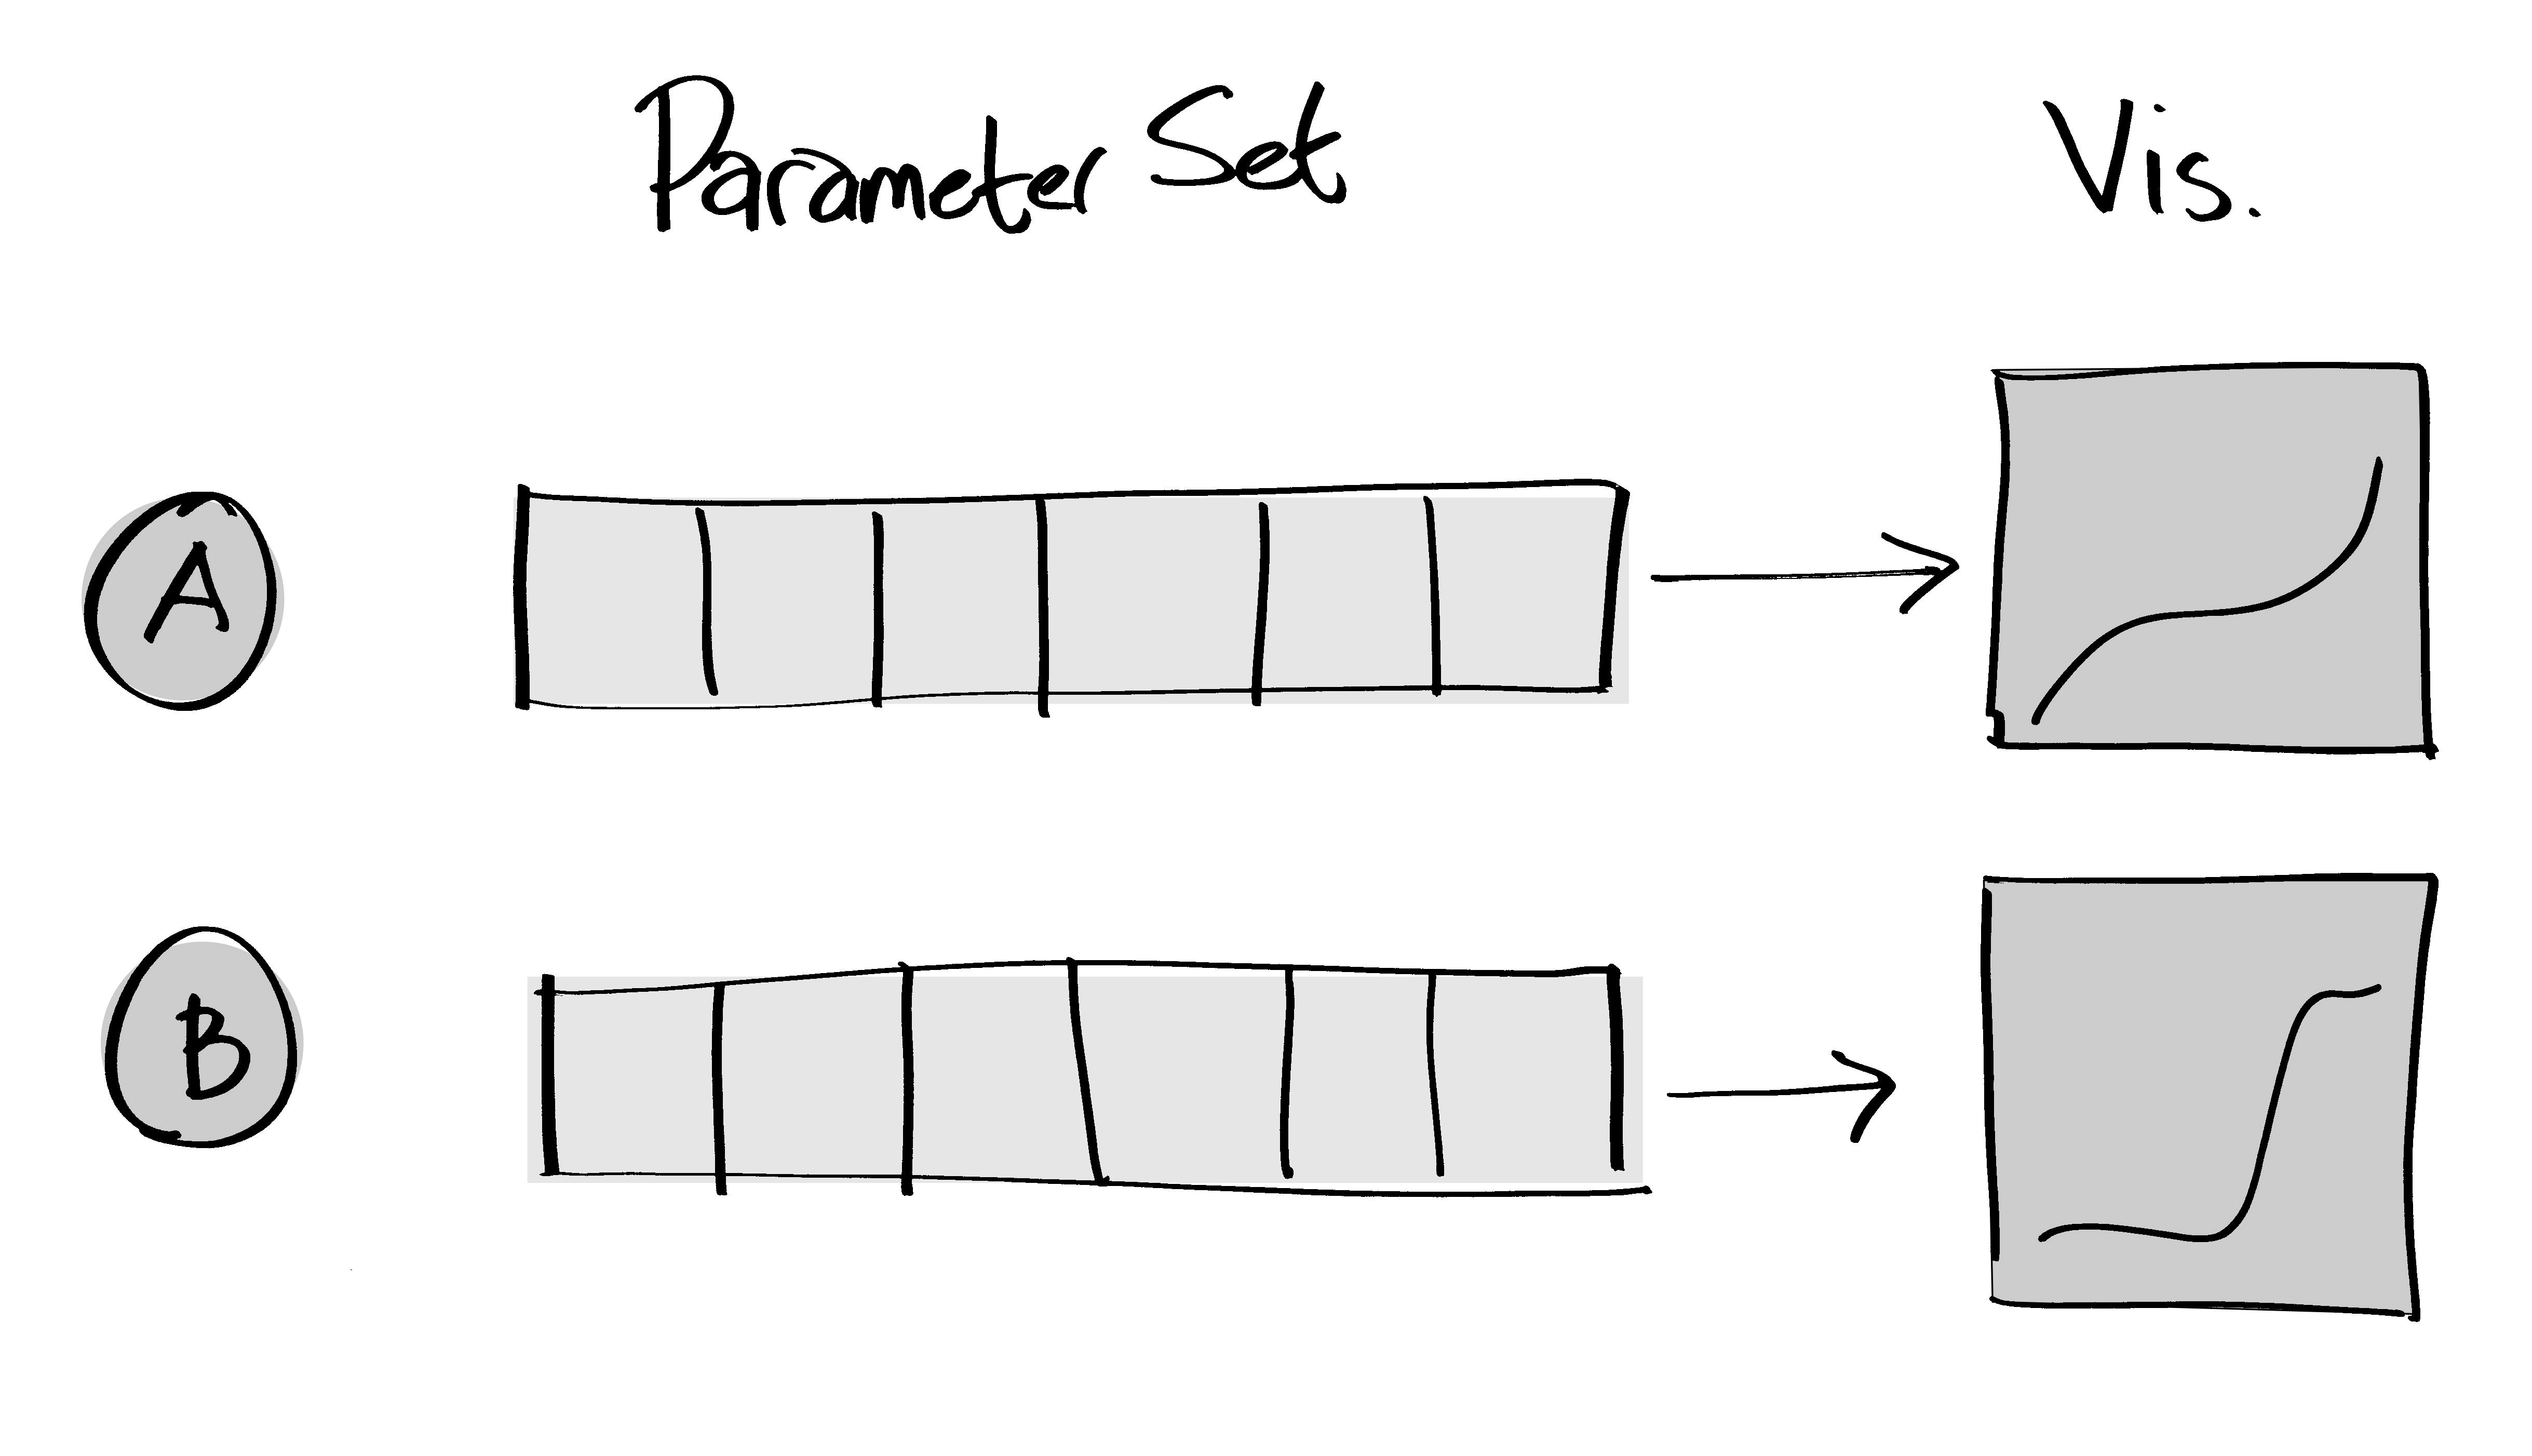
\includegraphics[width=0.8\textwidth]{img/parameter_set_diagram_filled}
\caption{
    Diagram showing a typical set of data that a scientist has for an experiment or simulations. Some set of parameters (A or B) has been used to create a visualization - a graph, an image captured from a sensor, or other data. These parameter sets can include, for example, settings on an experimental machine, inputs to a simulation, or measurements taken by a sensor. Each one of the parameter sets thus defines a unique result. Taken together, a set of these parameter sets constitutes a database of results, and a scientist often tracks this database in a spreadsheet. These parameter set/image pairings form the basis for the simplest Spec D database.
}
\label{fig:parametersets}
\end{figure}




\newpage
\section{The Cinema D (\dietrich) v\version Specification}
\label{dietrich}
Cinema D (\dietrich) specification is a table-based data model for scientific
data. In version 1.1 of this specification, we take the simplest approach to
this new model, to simplify adoption and interaction with Cinema.

\subsection{Required Elements}

A Specification D version 1.1 Cinema database is directory that contains all of
the data in the database. The directory must have the following files.
Additional files or directories may be present, but they are ignored by Cinema.

\begin{itemize}
\item a directory named \texttt{\small database\_name.cdb} 
  ({\em database\_name} is the name of the database) containing:
\begin{itemize}
\item \texttt{\small data.csv}, a Comma Separated Value file. This file is
  specified in Section \ref{csv}. The presence of this specifically named file 
  indicates that this is a Spec D, version 1.1 Cinema database.
\item optional data files, referenced by the \texttt{\small data.csv} file.
\item additional files in the directory, ignored by this specification.
%\begin{comment}
%  {\em except} \texttt{\small data.json}. If \texttt{\small data.json} exists
%  in the root directory, then this defines a Spec D, version 2.0 Cinema 
%  database. \textbf{Do not have a file named \texttt{\small data.json} if you 
%  want this to be a Cinema D v1.1 database}.
%\end{comment}
\end{itemize}
\end{itemize}

%Cinema D v2.0, which is decribed in a separate document, is an extension to 
%existing v1.1 databases that provides additional capabilities. It is not 
%necessary to read the Cinema D v2.0 specification document or implement its
%capabilities for a Cinema D v1.1 reader and writer. As of this writing,
%the specification v2.0 is currently not available for download.


\subsection{The \texttt{data.csv} File}
\label{csv}
\input tex/csv

\section{Contacts and Further Information}
\label{contacts}
For further information, email the Cinema mailing list at \cinemaemail, or contact the authors of this document. Additional information is available at the Cinema website, \cinemawebsite.


\section{Changes from v1.1}
\label{changes}
Version 1.2 supersedes version 1.1. All v1.1 files are compliant v1.2 files,
but v1.2 files are not backwards compatible with v1.1. The following are the
changes and clarifications that have been made from v1.1 to v1.2:

\begin{itemize}
\item The first data line can contain (\texttt{\small NULL}) values, which
  means that \textbf{empty} data values can occur anywhere.
\item Clarifications made in section 3.2 under point 9.
\item Clarifications made to section 3.2.2 on data types, especially related
  to the support of \textbf{empty} values.
\end{itemize}


\section{Acknowledgements}
The image used on the cover page is a publicity photo of Marlene Dietrich for the film Shanghai Express (1932). This  photo is in the public domain \cite{dietrich}.

\newpage
\section{Bibliography}
\bibliographystyle{ieeetr}
\bibliography{bib/cinema}

\end{document}
